\documentclass[12pt]{article}
\usepackage{graphicx}
\usepackage {color}
\usepackage{pdfpages}
\usepackage{float}
\usepackage{changebar}
\usepackage{enumitem,amssymb}
\renewcommand{\familydefault}{\sfdefault}
\usepackage[margin=1.2in]{geometry}
\usepackage{graphicx}
\usepackage{wrapfig}
\usepackage[super]{cite}
\usepackage{subcaption}
\usepackage[table]{xcolor}
\usepackage{amsmath}
\usepackage[sort, numbers]{natbib}
\usepackage{multirow}
\usepackage{tabularx}
\usepackage{siunitx}

%%%%%%%%%%%%Defining the margins %%%%%%%%%%%%%%%%%%%%%
\textheight 9.in
\textwidth 6.5in
\topmargin -.5in
\oddsidemargin 0in
\setlength{\parskip}{\smallskipamount}

%%%%%%%%%%%%%%Specific Commands %%%%%%%%%%%%%%%%%%
\newcommand{\eg}{{\em e.g.,}}
\newcommand{\ie}{{\em i.e.,}}
\newcommand{\etc}{{\em etc.,}}
\newcommand{\etal}{{\em et al.}}
\newcommand{\degrees}{{$^{\circ}$}}
\newcommand{\fig}[1]{\textbf{Figure #1}}

%%%%%%%%%%%%%%%%%%%%%%%%%%%% Setting to control figure placement
% These determine the rules used to place floating objects like figures 
% They are only guides, but read the manual to see the effect of each.
\renewcommand{\topfraction}{.9}
\renewcommand{\bottomfraction}{.9}
\renewcommand{\textfraction}{.1}
\renewcommand{\familydefault}{\sfdefault} %setting the san serif font

%%%%%%%%%%%%%%%%%%%%%%%% Line spacing
% Use the following command for ``double'' spacing
%\setlength{\baselineskip}{1.2\baselineskip}
% and this one for an acceptable NIH spacing of 6lpi based on 11pt
%\setlength{\baselineskip}{.9\baselineskip}
% The baselineskip does not appear to work when we include a maketitle
% command in the main file.  Something there must set the line spacing
% If we use this next command, then things seem to work.
\renewcommand{\baselinestretch}{.9}

\setcounter{secnumdepth}{0} %make no numbers but have a table of contents


\begin{document}

\title{Lab 4: ECG Sim}
\author{Jake Bergquist, u6010393 }
\maketitle

\section{Introduction}
\par{}
Simulation based on models for the electrical activity of the heart are becoming a more and more common approach for the study and understanding of the way in which electrical potentials propagate from the heart to the torso surface as well as for the study of the underlying cardiac electro-physiology.[|<cite brett and such>] From this research effort, investigative tools such as ECGSIM have been developed to better interrogate the relationships between simulated cardiac action potentials and the resultant cardiac and torso electrical activity. 

In this lab our goal was to utilize ECGSIM to investigate the relationship between the characteristics of the heart such as the simulated action potentials on the heart surface and the resultant electrograms as measured on the heart and torso surface. In particular we focused on visualizing features of the action potential reflected on the epicardial and torso ecgs. ECGSIM allows the user a wide array of available manipulations of the underlying cardiac sources as well as several modalities of visualization. Using ECGSIM we can manipulate the upstroke time, amplitude, plateau duration, repolarization time, and baseline membrane voltage. ECG sim then uses these parameters the alter an underlying action potential model and generate transmembrane, and extracellular potentials for a heart beat. These simulated values zare the mapped onto a heart geometry and propagated through a torso geometry to the torso surface. The user can choose to view a rich amount of data in the form of potential maps, activation times, recovery times, ARI, and ecg leads from various torso recording locations. The changes made to the action poitentials can be made locally with a varying radius of effect even allowing control of transmural, epicardial or endocardial modification.

We utilized ECGsim to assess several action potential characteristics, specifically upstroke time, plateua duration and repolarization time, and how these effected potential maps, ARI, activation maps, BSP measurements, and ECG measurements.

\section{Methods}
\subsection{Question 1}
In order to investigate the relation ships between the activation of the ventricles as shown by the activation map and the potential distributions on the cardiac surface I first 


\section{Results}

\begin{figure}[H]
	
	\centering
	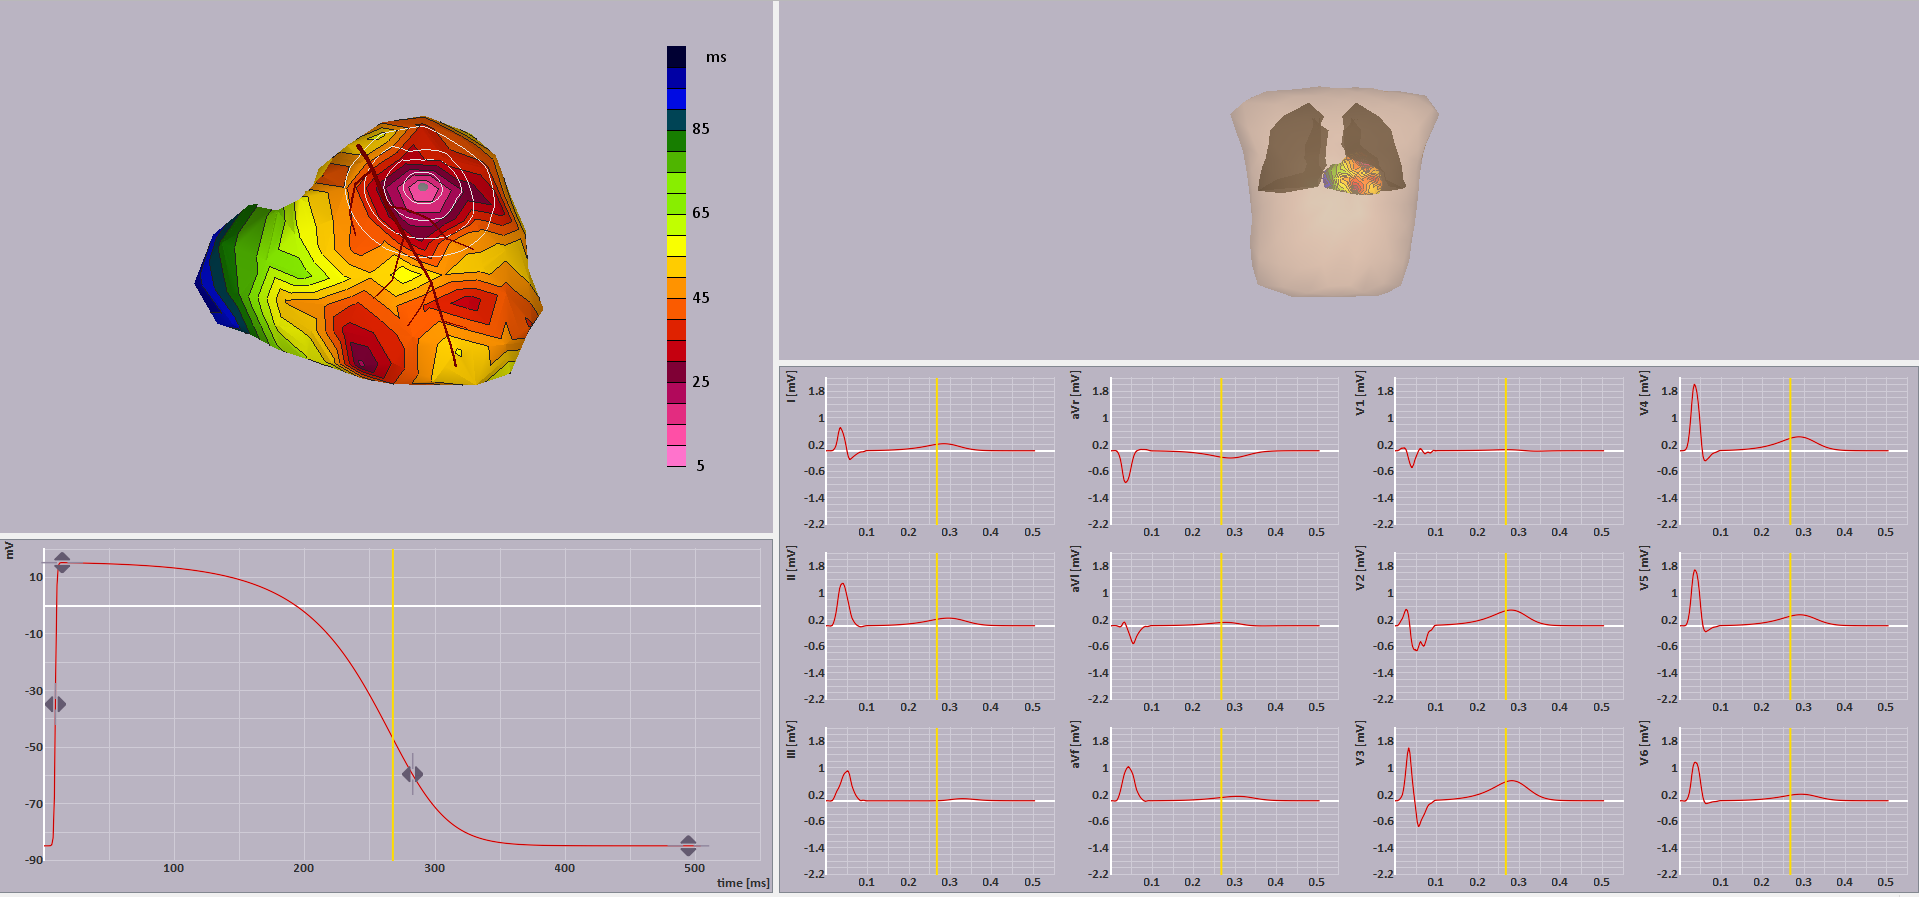
\includegraphics[width = .8\textwidth]{Figures/ActTimes.png}
	\caption{}
	\label{fig:ActT}
\end{figure}

\begin{figure}[H]
	
	\centering
	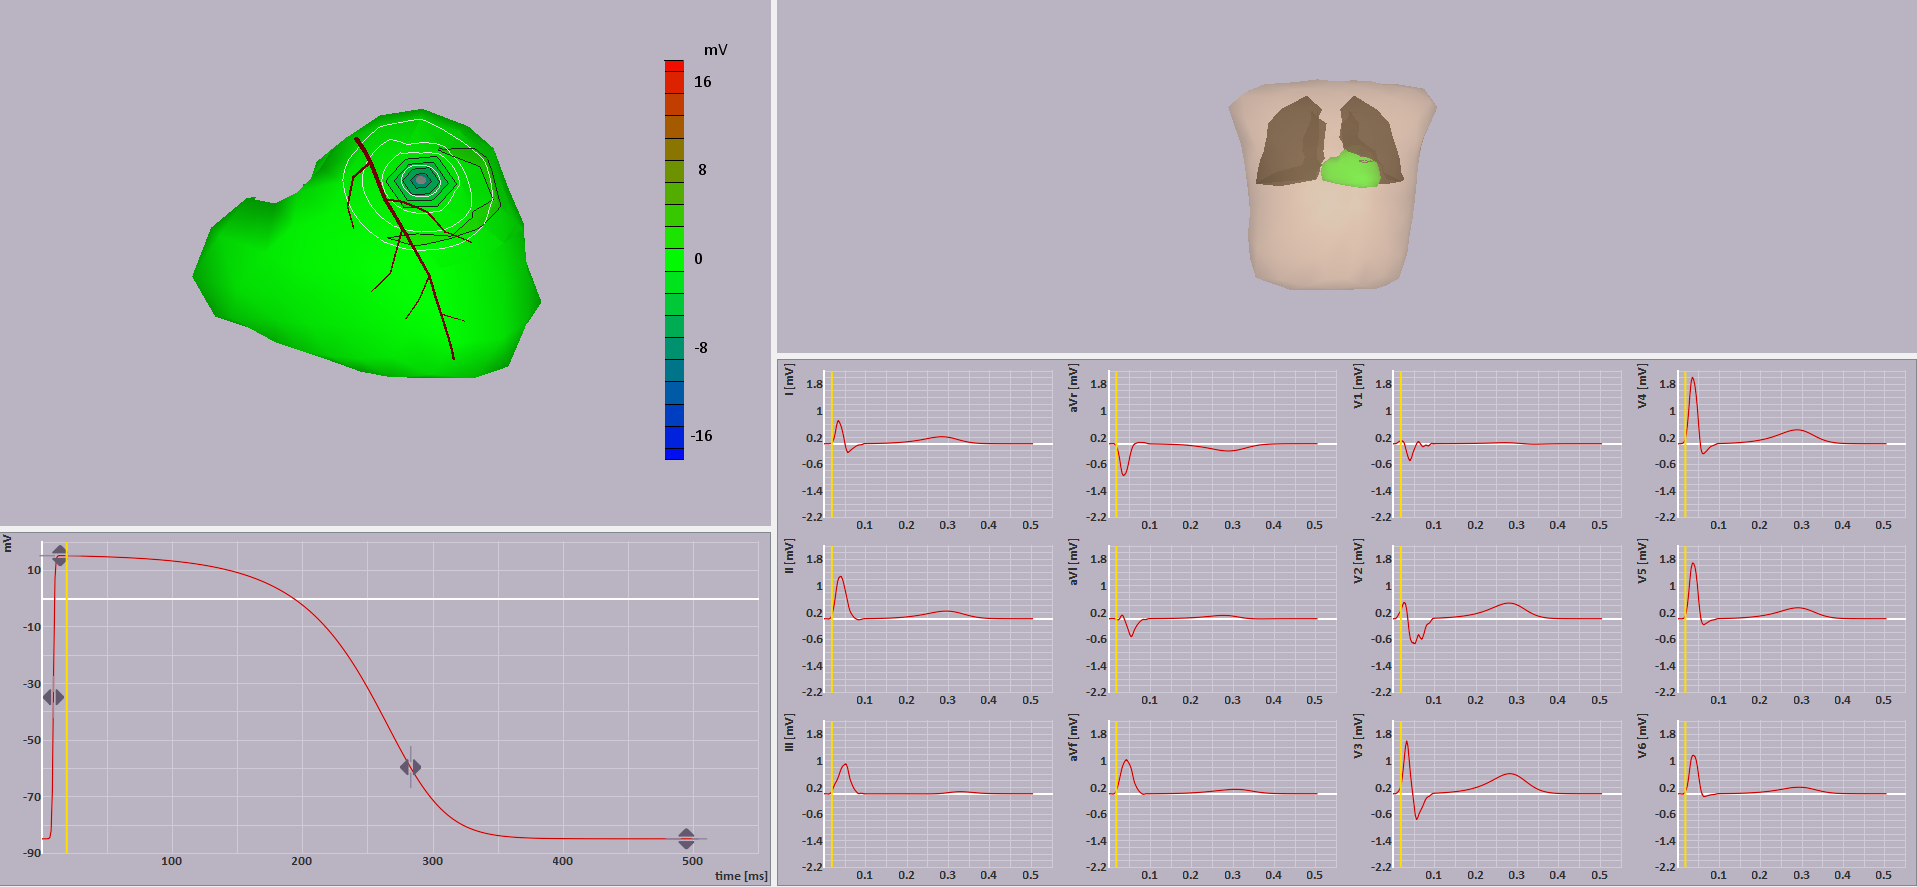
\includegraphics[width = .8\textwidth]{Figures/ActTimePotentials.png}
	\caption{}
	\label{fig:ActT_pot}
\end{figure}

\begin{figure}[H]
	
	\centering
	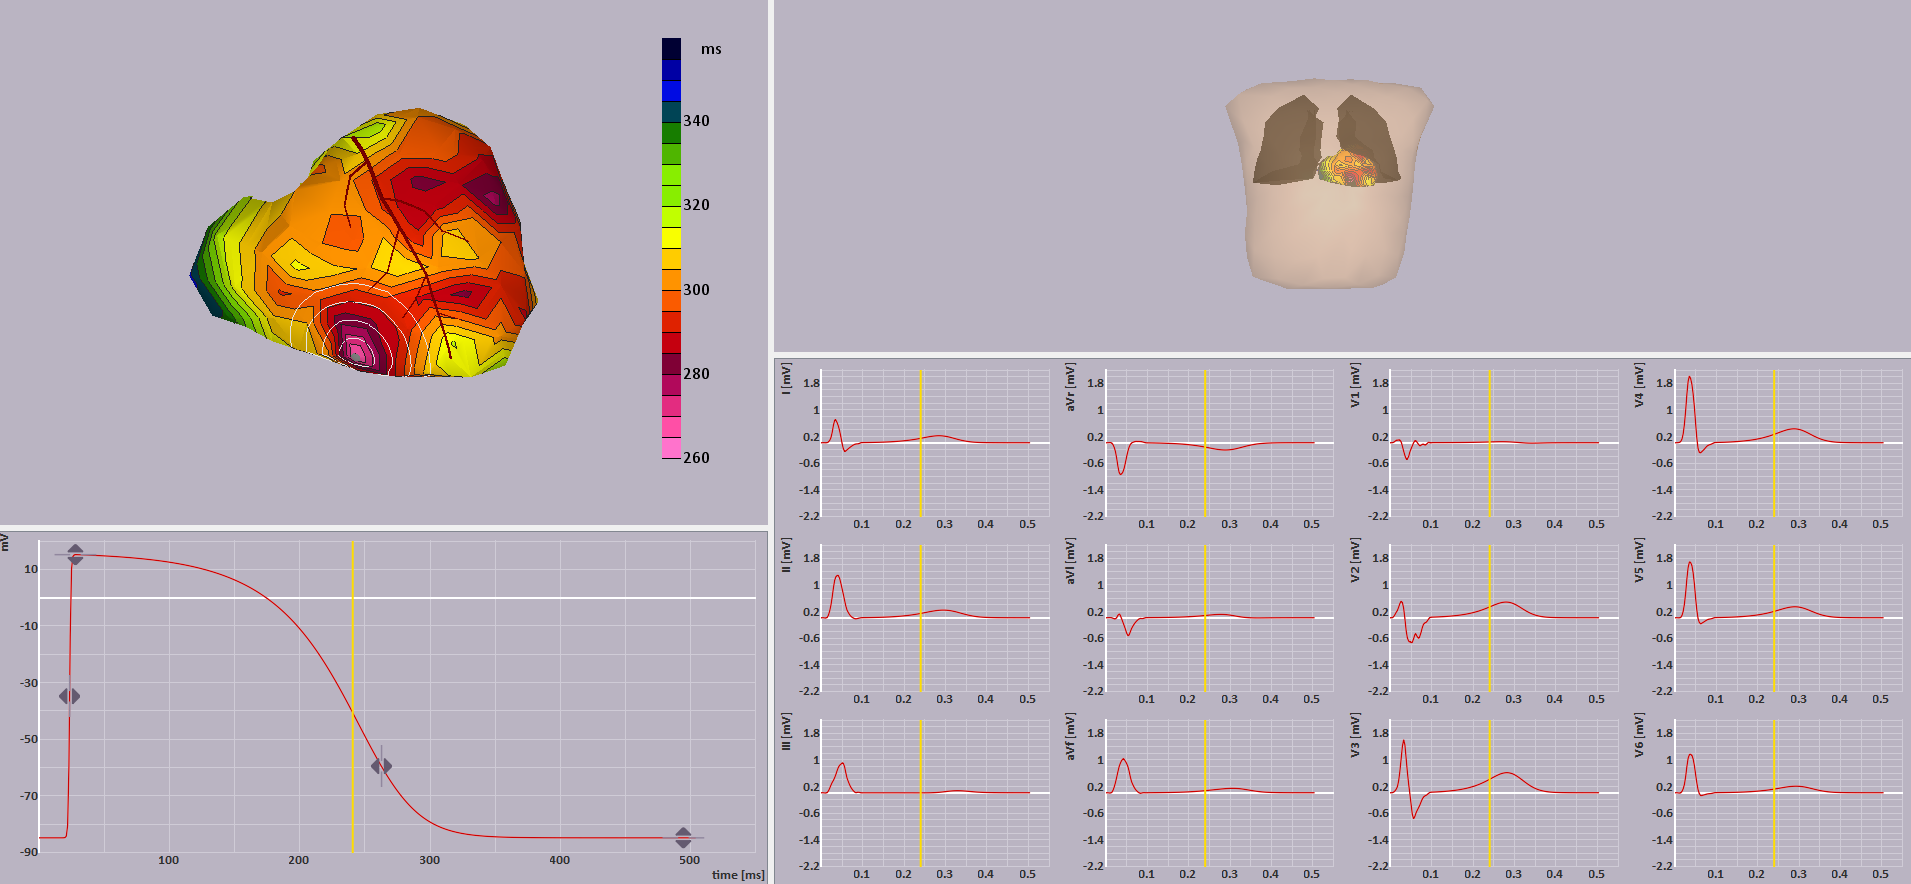
\includegraphics[width = .8\textwidth]{Figures/RecoTimes.png}
	\caption{}
	\label{fig:RecT}
\end{figure}

\begin{figure}[H]
	
	\centering
	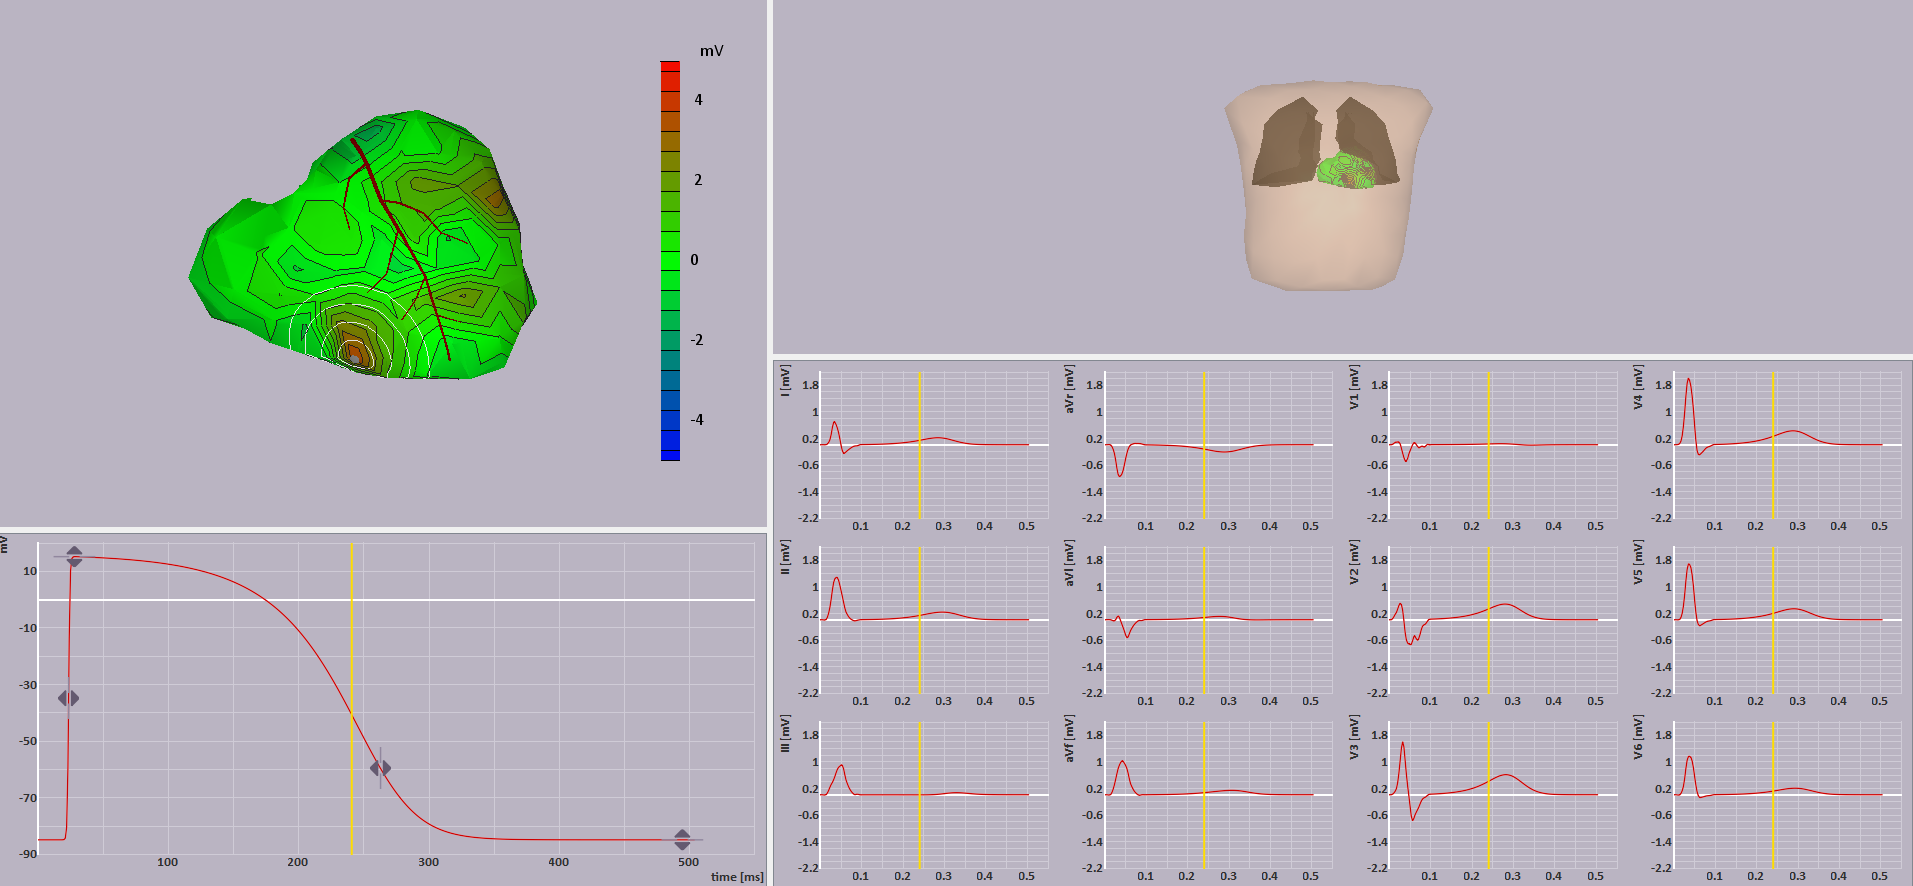
\includegraphics[width = .8\textwidth]{Figures/RecoPots.png}
	\caption{}
	\label{fig:RecT_pot}
\end{figure}

\begin{figure}[H]
	\centering
	\begin{subfigure}{0.45\textwidth}
		\centering
		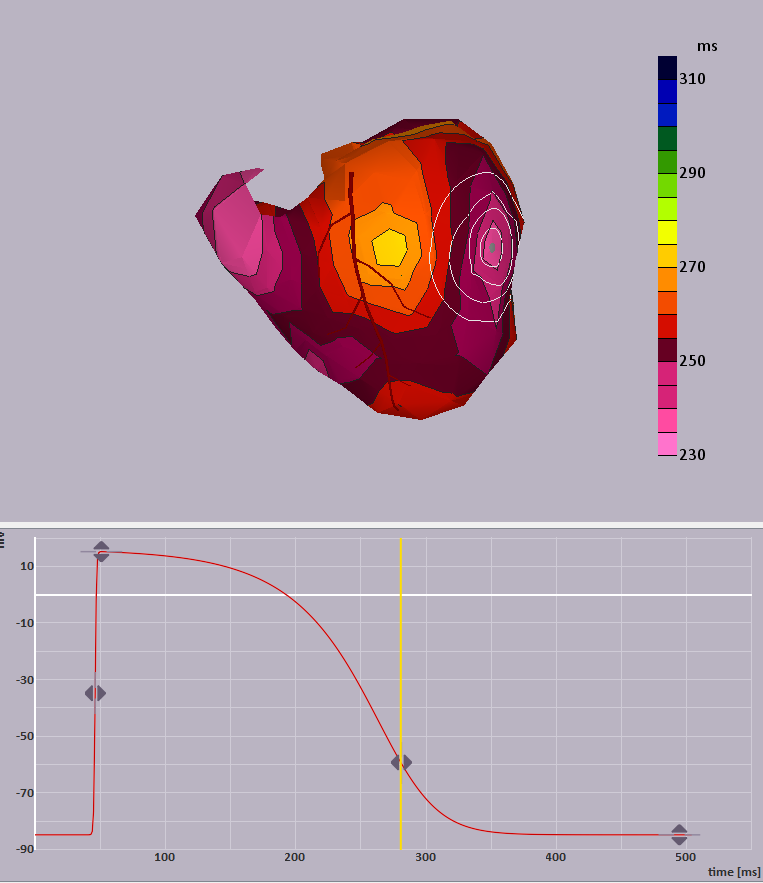
\includegraphics[width = \textwidth]{Figures/EpiADP.png}
		\caption{}
		\label{APD:epi}
	\end{subfigure}
	\begin{subfigure}{0.45\textwidth}
		\centering
		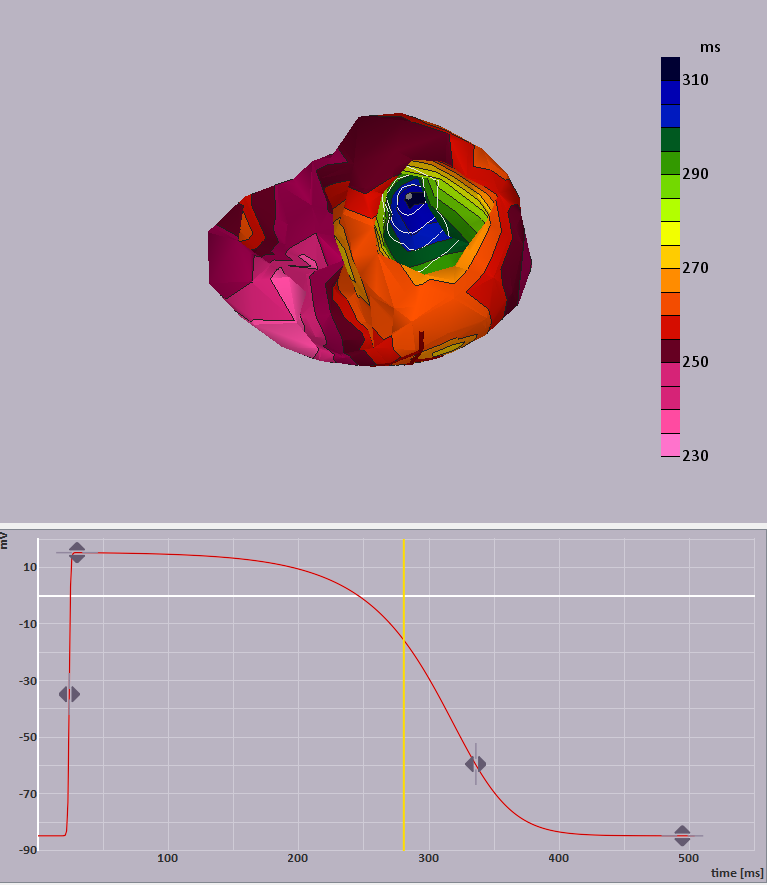
\includegraphics[width = \textwidth]{Figures/EndoADP.png}
		\caption{}
		\label{APD:endo}
	\end{subfigure}
	\begin{subfigure}{0.45\textwidth}
	\centering
	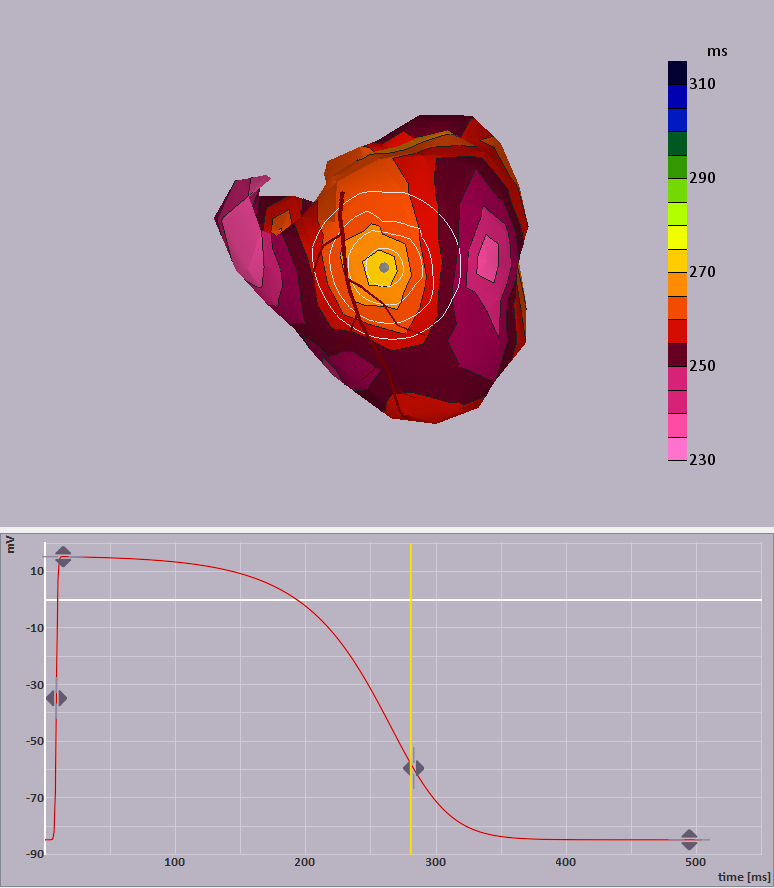
\includegraphics[width = \textwidth]{Figures/ADP_check1.png}
	\caption{}
	\label{APD:epi2}
	\end{subfigure}
	\begin{subfigure}{0.45\textwidth}
		\centering
		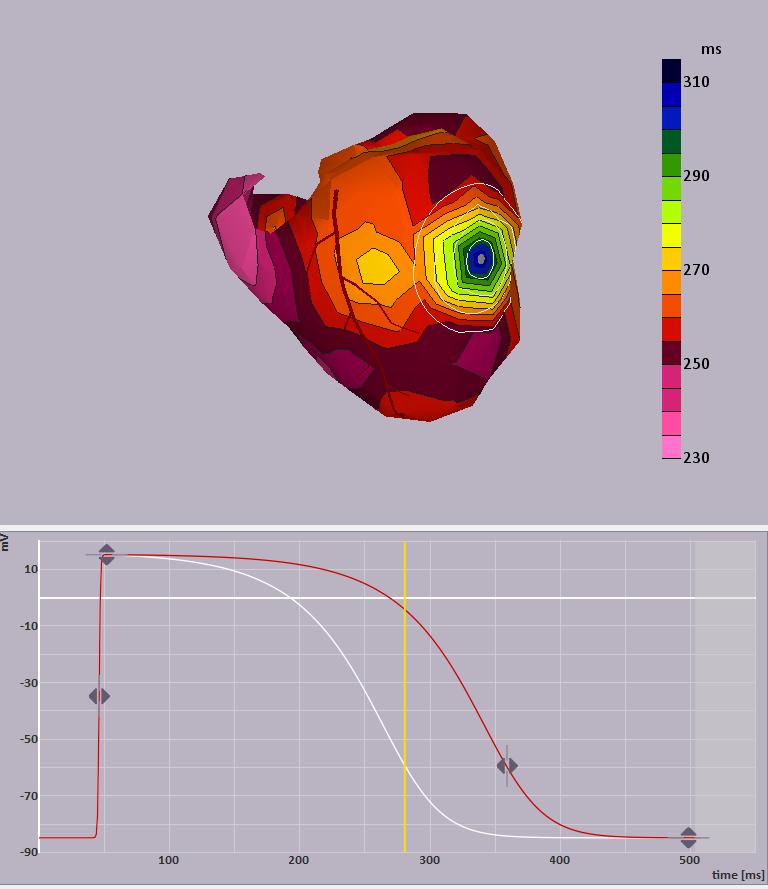
\includegraphics[width = \textwidth]{Figures/EpiChangedADP_1.png}
		\caption{}
		\label{APD:epichanged}
	\end{subfigure}

	\caption{}
	\label{fig:APD}
\end{figure}

\begin{figure}[H]
	\centering
	\begin{subfigure}{\textwidth}
		\centering
		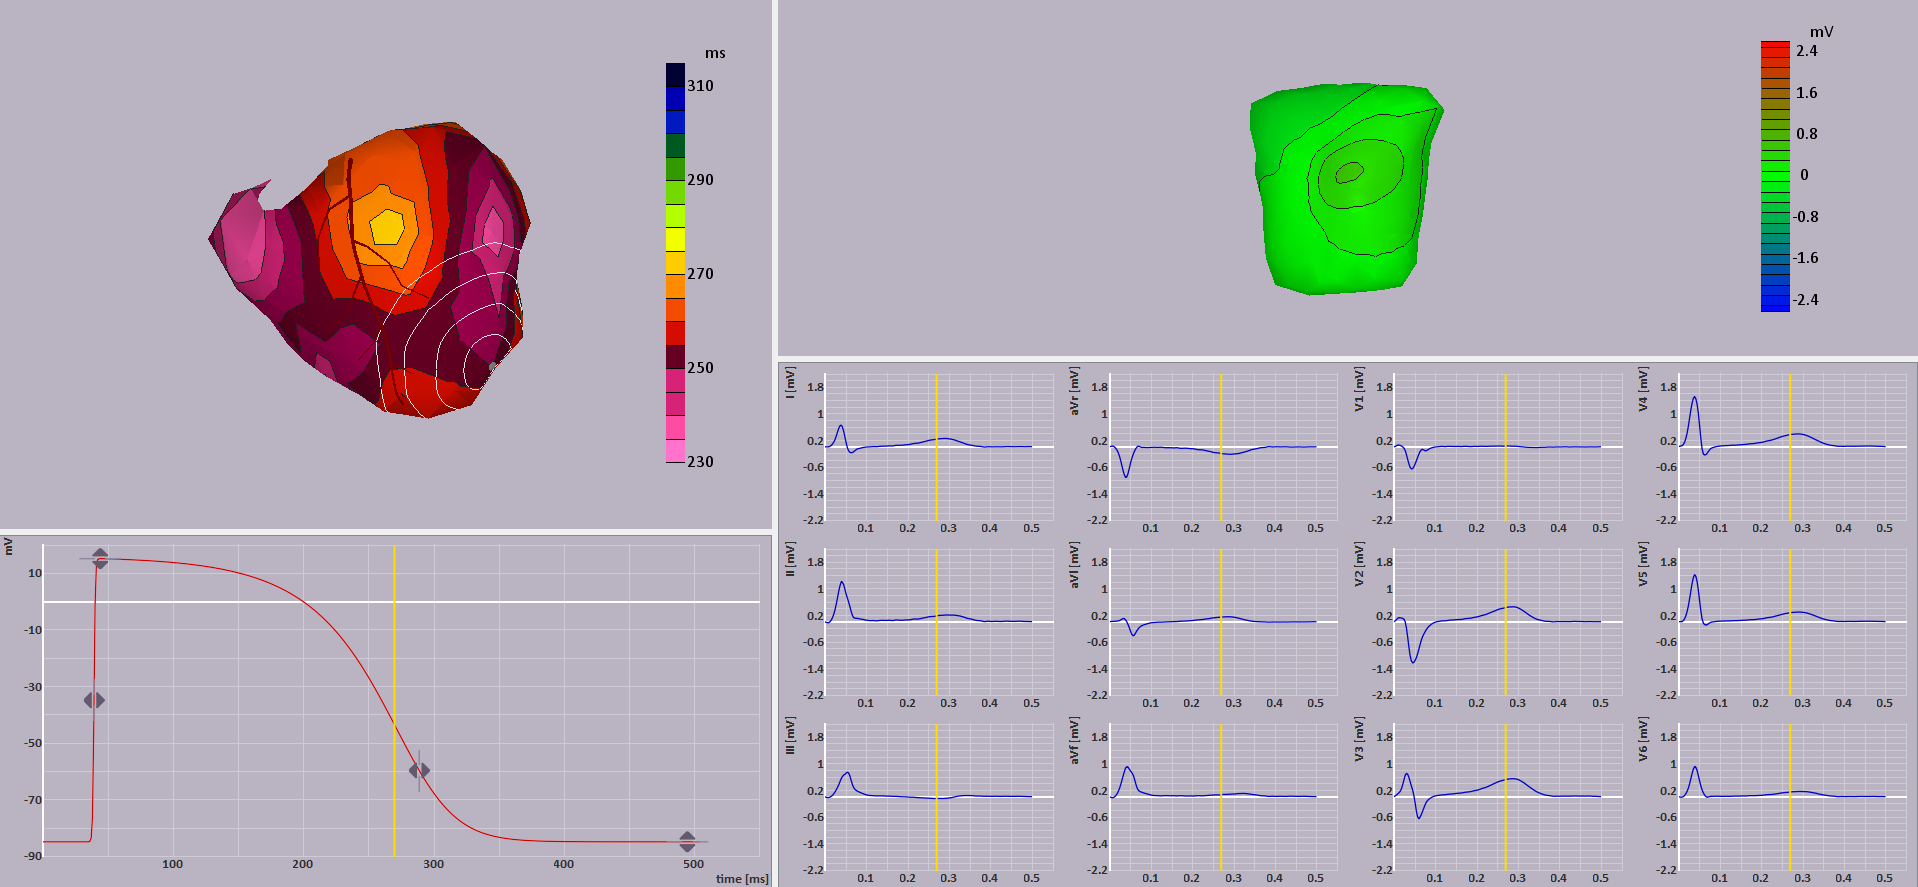
\includegraphics[width = \textwidth]{Figures/baselineBSO.png}
		\caption{}
		\label{BSP:Baseline}
	\end{subfigure}
	\begin{subfigure}{\textwidth}
		\centering
		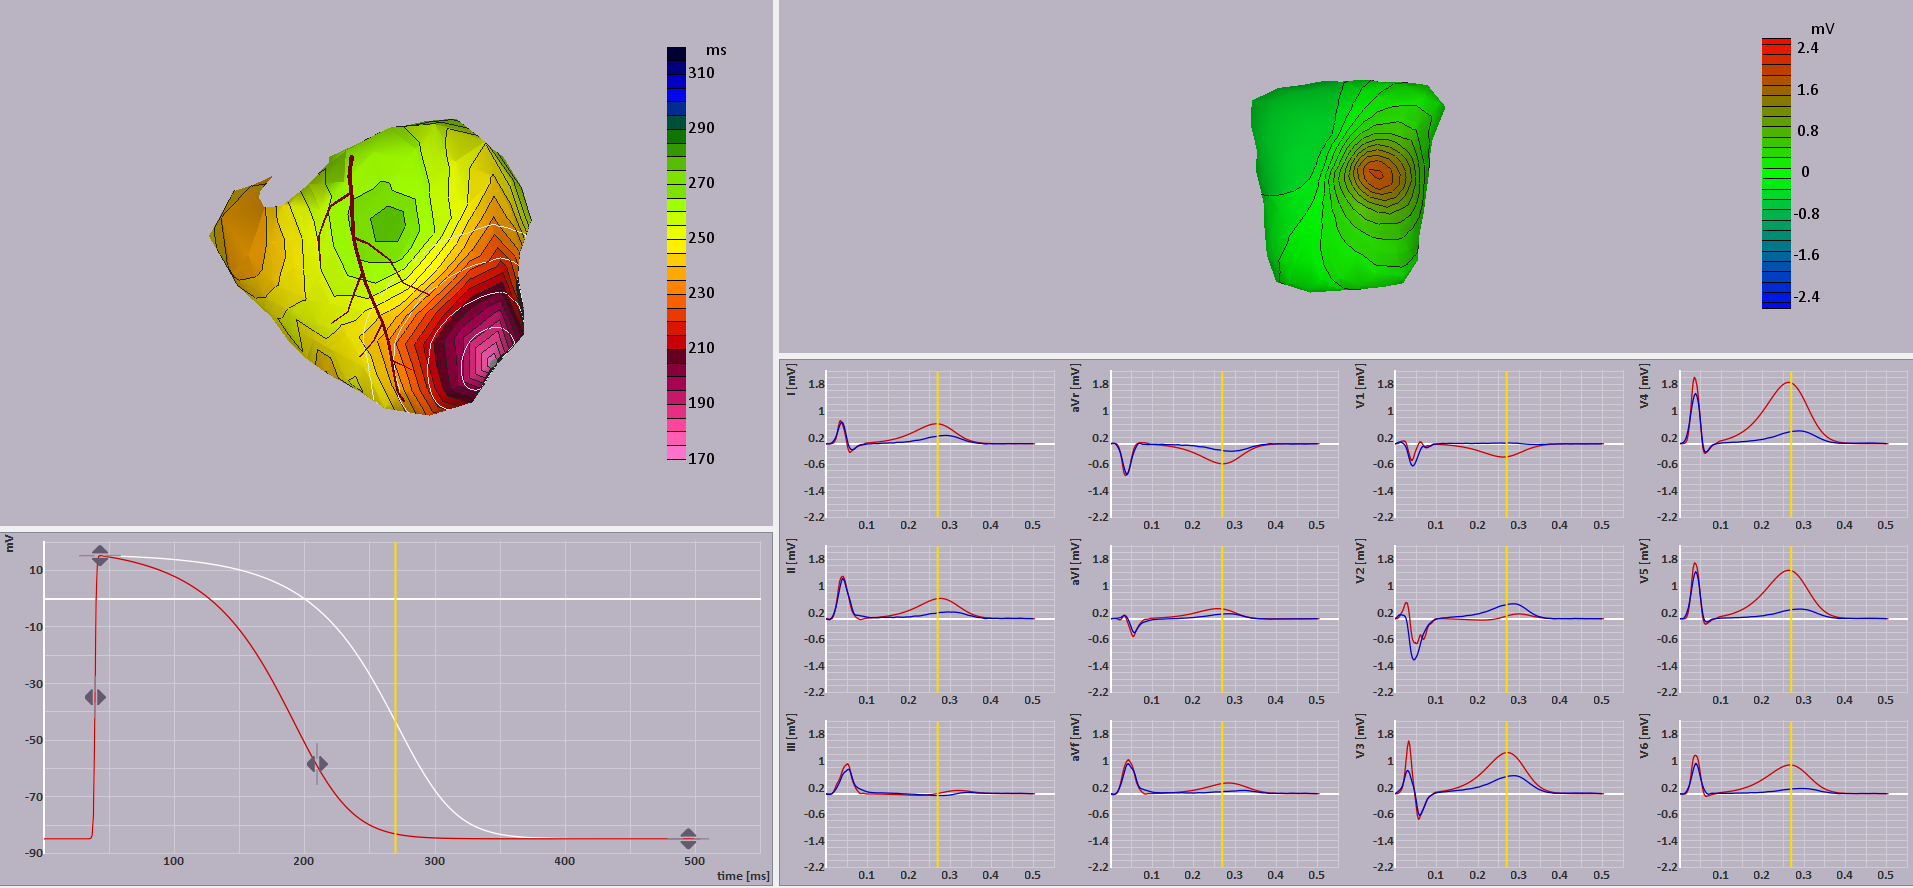
\includegraphics[width = \textwidth]{Figures/AltAPD_BSP.png}
		\caption{}
		\label{BSP:alt}
	\end{subfigure}

	
	\caption{}
	\label{fig:BSP}
\end{figure}

\section{Discussion}

%%%%%%%%%%%%%%%%%% Correct Bibliography Style

\bibliography{C:/Users/Jake/Documents/library}
\bibliographystyle{IEEEtran}


\end{document}








